\documentclass[12pt]{article}

%packages
%\usepackage{latexsym}
\usepackage{graphicx}
\usepackage{wrapfig}
\usepackage{color}
\usepackage{amsmath}
\usepackage{dsfont}
\usepackage{placeins}
\usepackage{amssymb}
\usepackage{skull}
\usepackage{enumerate}
\usepackage{soul}
\usepackage{alphalph}
\usepackage{hyperref}
\usepackage{enumerate}
\usepackage{listings}
\usepackage{multicol}
%\usepackage{fancyhdr}

%\fancyhf{} % clear all header and footers
%\renewcommand{\headrulewidth}{0pt} % remove the header rule
%\fancyfoot[LE, LO]{\thepage}


%\usepackage{pstricks,pst-node,pst-tree}

%\usepackage{algpseudocode}
%\usepackage{amsthm}
%\usepackage{hyperref}
%\usepackage{mathrsfs}
%\usepackage{amsfonts}
%\usepackage{bbding}
%\usepackage{listings}
%\usepackage{appendix}
\usepackage[margin=1in]{geometry}
%\geometry{papersize={8.5in,11in},total={6.5in,9in}}
%\usepackage{cancel}
%\usepackage{algorithmic, algorithm}

\definecolor{dkgreen}{rgb}{0,0.6,0}
\definecolor{gray}{rgb}{0.5,0.5,0.5}
\definecolor{mauve}{rgb}{0.58,0,0.82}
\lstset{ %
  language=R,                     % the language of the code
  basicstyle=\footnotesize,       % the size of the fonts that are used for the code
  numbers=left,                   % where to put the line-numbers
  numberstyle=\tiny\color{gray},  % the style that is used for the line-numbers
  stepnumber=1,                   % the step between two line-numbers. If it's 1, each line
                                  % will be numbered
  numbersep=5pt,                  % how far the line-numbers are from the code
  backgroundcolor=\color{white},  % choose the background color. You must add \usepackage{color}
  showspaces=false,               % show spaces adding particular underscores
  showstringspaces=false,         % underline spaces within strings
  showtabs=false,                 % show tabs within strings adding particular underscores
  frame=single,                   % adds a frame around the code
  rulecolor=\color{black},        % if not set, the frame-color may be changed on line-breaks within not-black text (e.g. commens (green here))
  tabsize=2,                      % sets default tabsize to 2 spaces
  captionpos=b,                   % sets the caption-position to bottom
  breaklines=true,                % sets automatic line breaking
  breakatwhitespace=false,        % sets if automatic breaks should only happen at whitespace
  title=\lstname,                 % show the filename of files included with \lstinputlisting;
                                  % also try caption instead of title
  keywordstyle=\color{black},      % keyword style
  commentstyle=\color{dkgreen},   % comment style
  stringstyle=\color{mauve},      % string literal style
  escapeinside={\%*}{*)},         % if you want to add a comment within your code
  morekeywords={*,...}            % if you want to add more keywords to the set
}

\newcommand{\qu}[1]{``#1''}
\newcommand{\spc}[1]{\\ \vspace{#1cm}}

\newcounter{probnum}
\setcounter{probnum}{1}

%create definition to allow local margin changes
\def\changemargin#1#2{\list{}{\rightmargin#2\leftmargin#1}\item[]}
\let\endchangemargin=\endlist 

%allow equations to span multiple pages
\allowdisplaybreaks

%define colors and color typesetting conveniences
\definecolor{gray}{rgb}{0.5,0.5,0.5}
\definecolor{black}{rgb}{0,0,0}
\definecolor{white}{rgb}{1,1,1}
\definecolor{blue}{rgb}{0.5,0.5,1}
\newcommand{\inblue}[1]{\color{blue}#1 \color{black}}
\definecolor{green}{rgb}{0.133,0.545,0.133}
\newcommand{\ingreen}[1]{\color{green}#1 \color{black}}
\definecolor{yellow}{rgb}{1,0.549,0}
\newcommand{\inyellow}[1]{\color{yellow}#1 \color{black}}
\definecolor{red}{rgb}{1,0.133,0.133}
\newcommand{\inred}[1]{\color{red}#1 \color{black}}
\definecolor{purple}{rgb}{0.58,0,0.827}
\newcommand{\inpurple}[1]{\color{purple}#1 \color{black}}
\definecolor{gray}{rgb}{0.5,0.5,0.5}
\newcommand{\ingray}[1]{\color{gray}#1 \color{black}}
\definecolor{backgcode}{rgb}{0.97,0.97,0.8}
\definecolor{Brown}{cmyk}{0,0.81,1,0.60}
\definecolor{OliveGreen}{cmyk}{0.64,0,0.95,0.40}
\definecolor{CadetBlue}{cmyk}{0.62,0.57,0.23,0}

%define new math operators
\DeclareMathOperator*{\argmax}{arg\,max~}
\DeclareMathOperator*{\argmin}{arg\,min~}
\DeclareMathOperator*{\argsup}{arg\,sup~}
\DeclareMathOperator*{\arginf}{arg\,inf~}
\DeclareMathOperator*{\convolution}{\text{\Huge{$\ast$}}}
\newcommand{\infconv}[2]{\convolution^\infty_{#1 = 1} #2}
%true functions

%%%% GENERAL SHORTCUTS

\makeatletter
\newalphalph{\alphmult}[mult]{\@alph}{26}
\renewcommand{\labelenumi}{(\alphmult{\value{enumi}})}
\renewcommand{\theenumi}{\AlphAlph{\value{enumi}}}
\makeatother
%shortcuts for pure typesetting conveniences
\newcommand{\bv}[1]{\boldsymbol{#1}}

%shortcuts for compound constants
\newcommand{\BetaDistrConst}{\dfrac{\Gamma(\alpha + \beta)}{\Gamma(\alpha)\Gamma(\beta)}}
\newcommand{\NormDistrConst}{\dfrac{1}{\sqrt{2\pi\sigma^2}}}

%shortcuts for conventional symbols
\newcommand{\tsq}{\tau^2}
\newcommand{\tsqh}{\hat{\tau}^2}
\newcommand{\sigsq}{\sigma^2}
\newcommand{\sigsqsq}{\parens{\sigma^2}^2}
\newcommand{\sigsqovern}{\dfrac{\sigsq}{n}}
\newcommand{\tausq}{\tau^2}
\newcommand{\tausqalpha}{\tau^2_\alpha}
\newcommand{\tausqbeta}{\tau^2_\beta}
\newcommand{\tausqsigma}{\tau^2_\sigma}
\newcommand{\betasq}{\beta^2}
\newcommand{\sigsqvec}{\bv{\sigma}^2}
\newcommand{\sigsqhat}{\hat{\sigma}^2}
\newcommand{\sigsqhatmlebayes}{\sigsqhat_{\text{Bayes, MLE}}}
\newcommand{\sigsqhatmle}[1]{\sigsqhat_{#1, \text{MLE}}}
\newcommand{\bSigma}{\bv{\Sigma}}
\newcommand{\bSigmainv}{\bSigma^{-1}}
\newcommand{\thetavec}{\bv{\theta}}
\newcommand{\thetahat}{\hat{\theta}}
\newcommand{\thetahatmm}{\hat{\theta}^{\mathrm{MM}}}
\newcommand{\thetahathatmm}{\thetahathat^{\mathrm{MM}}}
\newcommand{\thetahathatmle}{\thetahathat^{\mathrm{MLE}}}
\newcommand{\thetahatmle}{\hat{\theta}^{\mathrm{MLE}}}
\newcommand{\thetavechatmle}{\hat{\thetavec}^{\mathrm{MLE}}}
\newcommand{\muhat}{\hat{\mu}}
\newcommand{\musq}{\mu^2}
\newcommand{\muvec}{\bv{\mu}}
\newcommand{\muhatmle}{\muhat_{\text{MLE}}}
\newcommand{\lambdahat}{\hat{\lambda}}
\newcommand{\lambdahatmle}{\lambdahat_{\text{MLE}}}
\newcommand{\thetahatmap}{\hat{\theta}_{\mathrm{MAP}}}
\newcommand{\thetahatmmae}{\hat{\theta}_{\mathrm{MMAE}}}
\newcommand{\thetahatmmse}{\hat{\theta}_{\mathrm{MMSE}}}
\newcommand{\etavec}{\bv{\eta}}
\newcommand{\alphavec}{\bv{\alpha}}
\newcommand{\minimaxdec}{\delta^*_{\mathrm{mm}}}
\newcommand{\ybar}{\bar{y}}
\newcommand{\xbar}{\bar{x}}
\newcommand{\Xbar}{\bar{X}}
\newcommand{\iid}{~{\buildrel iid \over \sim}~}
\newcommand{\inddist}{~{\buildrel ind \over \sim}~}
\newcommand{\approxdist}{~{\buildrel \bv{\cdot} \over \sim}~}
\newcommand{\equalsindist}{~{\buildrel d \over =}~}
\newcommand{\loglik}[1]{\ell\parens{#1}}
\newcommand{\thetahatkminone}{\thetahat^{(k-1)}}
\newcommand{\thetahatkplusone}{\thetahat^{(k+1)}}
\newcommand{\thetahatk}{\thetahat^{(k)}}
\newcommand{\half}{\frac{1}{2}}
\newcommand{\third}{\frac{1}{3}}
\newcommand{\twothirds}{\frac{2}{3}}
\newcommand{\fourth}{\frac{1}{4}}
\newcommand{\fifth}{\frac{1}{5}}
\newcommand{\sixth}{\frac{1}{6}}

%shortcuts for vector and matrix notation
\newcommand{\A}{\bv{A}}
\newcommand{\At}{\A^T}
\newcommand{\Ainv}{\inverse{\A}}
\newcommand{\B}{\bv{B}}
\renewcommand{\b}{\bv{b}}
\renewcommand{\H}{\bv{H}}
\newcommand{\K}{\bv{K}}
\newcommand{\Kt}{\K^T}
\newcommand{\Kinv}{\inverse{K}}
\newcommand{\Kinvt}{(\Kinv)^T}
\newcommand{\M}{\bv{M}}
\newcommand{\Bt}{\B^T}
\newcommand{\Q}{\bv{Q}}
\newcommand{\Qt}{\Q^T}
\newcommand{\R}{\bv{R}}
\newcommand{\Rt}{\R^T}
\newcommand{\Z}{\bv{Z}}
\newcommand{\X}{\bv{X}}
\newcommand{\Xsub}{\X_{\text{(sub)}}}
\newcommand{\Xsubadj}{\X_{\text{(sub,adj)}}}
\newcommand{\I}{\bv{I}}
\newcommand{\Y}{\bv{Y}}
\newcommand{\sigsqI}{\sigsq\I}
\renewcommand{\P}{\bv{P}}
\newcommand{\Psub}{\P_{\text{(sub)}}}
\newcommand{\Pt}{\P^T}
\newcommand{\Pii}{P_{ii}}
\newcommand{\Pij}{P_{ij}}
\newcommand{\IminP}{(\I-\P)}
\newcommand{\Xt}{\bv{X}^T}
\newcommand{\XtX}{\Xt\X}
\newcommand{\XtXinv}{\parens{\Xt\X}^{-1}}
\newcommand{\XtXinvXt}{\XtXinv\Xt}
\newcommand{\XXtXinvXt}{\X\XtXinvXt}
\newcommand{\x}{\bv{x}}
\newcommand{\w}{\bv{w}}
\newcommand{\q}{\bv{q}}
\newcommand{\zerovec}{\bv{0}}
\newcommand{\onevec}{\bv{1}}
\newcommand{\oneton}{1, \ldots, n}
\newcommand{\yoneton}{y_1, \ldots, y_n}
\newcommand{\yonetonorder}{y_{(1)}, \ldots, y_{(n)}}
\newcommand{\Yoneton}{Y_1, \ldots, Y_n}
\newcommand{\iinoneton}{i \in \braces{\oneton}}
\newcommand{\onetom}{1, \ldots, m}
\newcommand{\jinonetom}{j \in \braces{\onetom}}
\newcommand{\xoneton}{x_1, \ldots, x_n}
\newcommand{\Xoneton}{X_1, \ldots, X_n}
\newcommand{\xt}{\x^T}
\newcommand{\y}{\bv{y}}
\newcommand{\yt}{\y^T}
\renewcommand{\c}{\bv{c}}
\newcommand{\ct}{\c^T}
\newcommand{\tstar}{\bv{t}^*}
\renewcommand{\u}{\bv{u}}
\renewcommand{\v}{\bv{v}}
\renewcommand{\a}{\bv{a}}
\newcommand{\s}{\bv{s}}
\newcommand{\yadj}{\y_{\text{(adj)}}}
\newcommand{\xjadj}{\x_{j\text{(adj)}}}
\newcommand{\xjadjM}{\x_{j \perp M}}
\newcommand{\yhat}{\hat{\y}}
\newcommand{\yhatsub}{\yhat_{\text{(sub)}}}
\newcommand{\yhatstar}{\yhat^*}
\newcommand{\yhatstarnew}{\yhatstar_{\text{new}}}
\newcommand{\z}{\bv{z}}
\newcommand{\zt}{\z^T}
\newcommand{\bb}{\bv{b}}
\newcommand{\bbt}{\bb^T}
\newcommand{\bbeta}{\bv{\beta}}
\newcommand{\beps}{\bv{\epsilon}}
\newcommand{\bepst}{\beps^T}
\newcommand{\e}{\bv{e}}
\newcommand{\Mofy}{\M(\y)}
\newcommand{\KofAlpha}{K(\alpha)}
\newcommand{\ellset}{\mathcal{L}}
\newcommand{\oneminalph}{1-\alpha}
\newcommand{\SSE}{\text{SSE}}
\newcommand{\SSEsub}{\text{SSE}_{\text{(sub)}}}
\newcommand{\MSE}{\text{MSE}}
\newcommand{\RMSE}{\text{RMSE}}
\newcommand{\SSR}{\text{SSR}}
\newcommand{\SST}{\text{SST}}
\newcommand{\JSest}{\delta_{\text{JS}}(\x)}
\newcommand{\Bayesest}{\delta_{\text{Bayes}}(\x)}
\newcommand{\EmpBayesest}{\delta_{\text{EmpBayes}}(\x)}
\newcommand{\BLUPest}{\delta_{\text{BLUP}}}
\newcommand{\MLEest}[1]{\hat{#1}_{\text{MLE}}}

%shortcuts for Linear Algebra stuff (i.e. vectors and matrices)
\newcommand{\twovec}[2]{\bracks{\begin{array}{c} #1 \\ #2 \end{array}}}
\newcommand{\threevec}[3]{\bracks{\begin{array}{c} #1 \\ #2 \\ #3 \end{array}}}
\newcommand{\fivevec}[5]{\bracks{\begin{array}{c} #1 \\ #2 \\ #3 \\ #4 \\ #5 \end{array}}}
\newcommand{\twobytwomat}[4]{\bracks{\begin{array}{cc} #1 & #2 \\ #3 & #4 \end{array}}}
\newcommand{\threebytwomat}[6]{\bracks{\begin{array}{cc} #1 & #2 \\ #3 & #4 \\ #5 & #6 \end{array}}}

%shortcuts for conventional compound symbols
\newcommand{\thetainthetas}{\theta \in \Theta}
\newcommand{\reals}{\mathbb{R}}
\newcommand{\complexes}{\mathbb{C}}
\newcommand{\rationals}{\mathbb{Q}}
\newcommand{\integers}{\mathbb{Z}}
\newcommand{\naturals}{\mathbb{N}}
\newcommand{\forallninN}{~~\forall n \in \naturals}
\newcommand{\forallxinN}[1]{~~\forall #1 \in \reals}
\newcommand{\matrixdims}[2]{\in \reals^{\,#1 \times #2}}
\newcommand{\inRn}[1]{\in \reals^{\,#1}}
\newcommand{\mathimplies}{\quad\Rightarrow\quad}
\newcommand{\mathlogicequiv}{\quad\Leftrightarrow\quad}
\newcommand{\eqncomment}[1]{\quad \text{(#1)}}
\newcommand{\limitn}{\lim_{n \rightarrow \infty}}
\newcommand{\limitN}{\lim_{N \rightarrow \infty}}
\newcommand{\limitd}{\lim_{d \rightarrow \infty}}
\newcommand{\limitt}{\lim_{t \rightarrow \infty}}
\newcommand{\limitsupn}{\limsup_{n \rightarrow \infty}~}
\newcommand{\limitinfn}{\liminf_{n \rightarrow \infty}~}
\newcommand{\limitk}{\lim_{k \rightarrow \infty}}
\newcommand{\limsupn}{\limsup_{n \rightarrow \infty}}
\newcommand{\limsupk}{\limsup_{k \rightarrow \infty}}
\newcommand{\floor}[1]{\left\lfloor #1 \right\rfloor}
\newcommand{\ceil}[1]{\left\lceil #1 \right\rceil}

%shortcuts for environments
\newcommand{\beqn}{\vspace{-0.25cm}\begin{eqnarray*}}
\newcommand{\eeqn}{\end{eqnarray*}}
\newcommand{\bneqn}{\vspace{-0.25cm}\begin{eqnarray}}
\newcommand{\eneqn}{\end{eqnarray}}
\newcommand{\benum}{\begin{itemize}}
\newcommand{\eenum}{\end{itemize}}

%shortcuts for mini environments
\newcommand{\parens}[1]{\left(#1\right)}
\newcommand{\squared}[1]{\parens{#1}^2}
\newcommand{\tothepow}[2]{\parens{#1}^{#2}}
\newcommand{\prob}[1]{\mathbb{P}\parens{#1}}
\newcommand{\littleo}[1]{o\parens{#1}}
\newcommand{\bigo}[1]{O\parens{#1}}
\newcommand{\Lp}[1]{\mathbb{L}^{#1}}
\renewcommand{\arcsin}[1]{\text{arcsin}\parens{#1}}
\newcommand{\prodonen}[2]{\bracks{\prod_{#1=1}^n #2}}
\newcommand{\mysum}[4]{\sum_{#1=#2}^{#3} #4}
\newcommand{\sumonen}[2]{\sum_{#1=1}^n #2}
\newcommand{\infsum}[2]{\sum_{#1=1}^\infty #2}
\newcommand{\infprod}[2]{\prod_{#1=1}^\infty #2}
\newcommand{\infunion}[2]{\bigcup_{#1=1}^\infty #2}
\newcommand{\infinter}[2]{\bigcap_{#1=1}^\infty #2}
\newcommand{\infintegral}[2]{\int^\infty_{-\infty} #2 ~\text{d}#1}
\newcommand{\supthetas}[1]{\sup_{\thetainthetas}\braces{#1}}
\newcommand{\bracks}[1]{\left[#1\right]}
\newcommand{\braces}[1]{\left\{#1\right\}}
\newcommand{\angbraces}[1]{\left<#1\right>}
\newcommand{\set}[1]{\left\{#1\right\}}
\newcommand{\abss}[1]{\left|#1\right|}
\newcommand{\norm}[1]{\left|\left|#1\right|\right|}
\newcommand{\normsq}[1]{\norm{#1}^2}
\newcommand{\inverse}[1]{\parens{#1}^{-1}}
\newcommand{\rowof}[2]{\parens{#1}_{#2\cdot}}

%shortcuts for functionals
\newcommand{\realcomp}[1]{\text{Re}\bracks{#1}}
\newcommand{\imagcomp}[1]{\text{Im}\bracks{#1}}
\newcommand{\range}[1]{\text{range}\bracks{#1}}
\newcommand{\colsp}[1]{\text{colsp}\bracks{#1}}
\newcommand{\rowsp}[1]{\text{rowsp}\bracks{#1}}
\newcommand{\tr}[1]{\text{tr}\bracks{#1}}
\newcommand{\rank}[1]{\text{rank}\bracks{#1}}
\newcommand{\proj}[2]{\text{Proj}_{#1}\bracks{#2}}
\newcommand{\projcolspX}[1]{\text{Proj}_{\colsp{\X}}\bracks{#1}}
\newcommand{\median}[1]{\text{median}\bracks{#1}}
\newcommand{\mean}[1]{\text{mean}\bracks{#1}}
\newcommand{\dime}[1]{\text{dim}\bracks{#1}}
\renewcommand{\det}[1]{\text{det}\bracks{#1}}
\newcommand{\expe}[1]{\mathbb{E}\bracks{#1}}
\newcommand{\expeabs}[1]{\expe{\abss{#1}}}
\newcommand{\expesub}[2]{\mathbb{E}_{#1}\bracks{#2}}
\newcommand{\cexpesub}[3]{\mathbb{E}_{#1}\bracks{#2~|~#3}}
\newcommand{\indic}[1]{\mathds{1}_{#1}}
\newcommand{\var}[1]{\mathbb{V}\text{ar}\bracks{#1}}
\newcommand{\mse}[1]{\mathbb{M}\text{SE}\bracks{#1}}
\newcommand{\sd}[1]{\mathbb{S}\text{D}\bracks{#1}}
\newcommand{\support}[1]{\mathbb{S}_{#1}}
\newcommand{\cov}[2]{\mathbb{C}\text{ov}\bracks{#1, #2}}
\newcommand{\corr}[2]{\mathbb{C}\text{orr}\bracks{#1, #2}}
\newcommand{\se}[1]{\text{SE}\bracks{#1}}
\newcommand{\seest}[1]{\hat{\text{SE}}\bracks{#1}}
\newcommand{\bias}[1]{\mathbb{B}\text{ias}\bracks{#1}}
\newcommand{\partialop}[2]{\dfrac{\partial}{\partial #1}\bracks{#2}}
\newcommand{\secpartialop}[2]{\dfrac{\partial^2}{\partial #1^2}\bracks{#2}}
\newcommand{\mixpartialop}[3]{\dfrac{\partial^2}{\partial #1 \partial #2}\bracks{#3}}

%shortcuts for functions
\renewcommand{\exp}[1]{\mathrm{exp}\parens{#1}}
\renewcommand{\cos}[1]{\text{cos}\parens{#1}}
\renewcommand{\sin}[1]{\text{sin}\parens{#1}}
\newcommand{\sign}[1]{\text{sign}\parens{#1}}
\newcommand{\are}[1]{\mathrm{ARE}\parens{#1}}
\newcommand{\natlog}[1]{\ln\parens{#1}}
\newcommand{\oneover}[1]{\frac{1}{#1}}
\newcommand{\overtwo}[1]{\frac{#1}{2}}
\newcommand{\overn}[1]{\frac{#1}{n}}
\newcommand{\oversqrtn}[1]{\frac{#1}{\sqrt{n}}}
\newcommand{\oneoversqrt}[1]{\oneover{\sqrt{#1}}}
\newcommand{\sqd}[1]{\parens{#1}^2}
\newcommand{\loss}[1]{\ell\parens{\theta, #1}}
\newcommand{\losstwo}[2]{\ell\parens{#1, #2}}
\newcommand{\cf}{\phi(t)}

%English language specific shortcuts
\newcommand{\ie}{\textit{i.e.} }
\newcommand{\AKA}{\textit{AKA} }
\renewcommand{\iff}{\textit{iff}}
\newcommand{\eg}{\textit{e.g.} }
\renewcommand{\st}{\textit{s.t.} }
\newcommand{\wrt}{\textit{w.r.t.} }
\newcommand{\mathst}{~~\text{\st}~~}
\newcommand{\mathand}{~~\text{and}~~}
\newcommand{\ala}{\textit{a la} }
\newcommand{\ppp}{posterior predictive p-value}
\newcommand{\dd}{dataset-to-dataset}

%shortcuts for distribution titles
\newcommand{\logistic}[2]{\mathrm{Logistic}\parens{#1,\,#2}}
\newcommand{\bernoulli}[1]{\mathrm{Bernoulli}\parens{#1}}
\newcommand{\betanot}[2]{\mathrm{Beta}\parens{#1,\,#2}}
\newcommand{\stdbetanot}{\betanot{\alpha}{\beta}}
\newcommand{\multnormnot}[3]{\mathcal{N}_{#1}\parens{#2,\,#3}}
\newcommand{\normnot}[2]{\mathcal{N}\parens{#1,\,#2}}
\newcommand{\classicnormnot}{\normnot{\mu}{\sigsq}}
\newcommand{\stdnormnot}{\normnot{0}{1}}
\newcommand{\uniform}[2]{\mathrm{U}\parens{#1,\,#2}}
\newcommand{\stduniform}{\uniform{0}{1}}
\newcommand{\exponential}[1]{\mathrm{Exp}\parens{#1}}
\newcommand{\geometric}[1]{\mathrm{Geometric}\parens{#1}}
\newcommand{\gammadist}[2]{\mathrm{Gamma}\parens{#1, #2}}
\newcommand{\negbin}[2]{\mathrm{NegBin}\parens{#1, #2}}
\newcommand{\poisson}[1]{\mathrm{Poisson}\parens{#1}}
\newcommand{\binomial}[2]{\mathrm{Binomial}\parens{#1,\,#2}}
\newcommand{\erlang}[2]{\mathrm{Erlang}\parens{#1,\,#2}}
\newcommand{\rayleigh}[1]{\mathrm{Rayleigh}\parens{#1}}
\newcommand{\multinomial}[3]{\mathrm{Multinom}_{#1}\parens{#2,\,#3}}
\newcommand{\gammanot}[2]{\mathrm{Gamma}\parens{#1,\,#2}}
\newcommand{\cauchynot}[2]{\text{Cauchy}\parens{#1,\,#2}}
\newcommand{\invchisqnot}[1]{\text{Inv}\chisq{#1}}
\newcommand{\invscaledchisqnot}[2]{\text{ScaledInv}\ncchisq{#1}{#2}}
\newcommand{\invgammanot}[2]{\text{InvGamma}\parens{#1,\,#2}}
\newcommand{\chisq}[1]{\chi^2_{#1}}
\newcommand{\ncchisq}[2]{\chi^2_{#1}\parens{#2}}
\newcommand{\ncF}[3]{F_{#1,#2}\parens{#3}}

%shortcuts for PDF's of common distributions
\newcommand{\logisticpdf}[3]{\oneover{#3}\dfrac{\exp{-\dfrac{#1 - #2}{#3}}}{\parens{1+\exp{-\dfrac{#1 - #2}{#3}}}^2}}
\newcommand{\betapdf}[3]{\dfrac{\Gamma(#2 + #3)}{\Gamma(#2)\Gamma(#3)}#1^{#2-1} (1-#1)^{#3-1}}
\newcommand{\normpdf}[3]{\frac{1}{\sqrt{2\pi#3}}\exp{-\frac{1}{2#3}(#1 - #2)^2}}
\newcommand{\normpdfvarone}[2]{\dfrac{1}{\sqrt{2\pi}}e^{-\half(#1 - #2)^2}}
\newcommand{\chisqpdf}[2]{\dfrac{1}{2^{#2/2}\Gamma(#2/2)}\; {#1}^{#2/2-1} e^{-#1/2}}
\newcommand{\invchisqpdf}[2]{\dfrac{2^{-\overtwo{#1}}}{\Gamma(#2/2)}\,{#1}^{-\overtwo{#2}-1}  e^{-\oneover{2 #1}}}
\newcommand{\uniformdiscrete}[1]{\mathrm{Uniform}\parens{\braces{#1}}}
\newcommand{\exponentialpdf}[2]{#2\exp{-#2#1}}
\newcommand{\poissonpdf}[2]{\dfrac{e^{-#1} #1^{#2}}{#2!}}
\newcommand{\binomialpdf}[3]{\binom{#2}{#1}#3^{#1}(1-#3)^{#2-#1}}
\newcommand{\rayleighpdf}[2]{\dfrac{#1}{#2^2}\exp{-\dfrac{#1^2}{2 #2^2}}}
\newcommand{\gammapdf}[3]{\dfrac{#3^#2}{\Gamma\parens{#2}}#1^{#2-1}\exp{-#3 #1}}
\newcommand{\cauchypdf}[3]{\oneover{\pi} \dfrac{#3}{\parens{#1-#2}^2 + #3^2}}
\newcommand{\Gammaf}[1]{\Gamma\parens{#1}}

%shortcuts for miscellaneous typesetting conveniences
\newcommand{\notesref}[1]{\marginpar{\color{gray}\tt #1\color{black}}}

%%%% DOMAIN-SPECIFIC SHORTCUTS

%Real analysis related shortcuts
\newcommand{\zeroonecl}{\bracks{0,1}}
\newcommand{\forallepsgrzero}{\forall \epsilon > 0~~}
\newcommand{\lessthaneps}{< \epsilon}
\newcommand{\fraccomp}[1]{\text{frac}\bracks{#1}}

%Bayesian related shortcuts
\newcommand{\yrep}{y^{\text{rep}}}
\newcommand{\yrepisq}{(\yrep_i)^2}
\newcommand{\yrepvec}{\bv{y}^{\text{rep}}}


%Probability shortcuts
\newcommand{\SigField}{\mathcal{F}}
\newcommand{\ProbMap}{\mathcal{P}}
\newcommand{\probtrinity}{\parens{\Omega, \SigField, \ProbMap}}
\newcommand{\convp}{~{\buildrel p \over \rightarrow}~}
\newcommand{\convLp}[1]{~{\buildrel \Lp{#1} \over \rightarrow}~}
\newcommand{\nconvp}{~{\buildrel p \over \nrightarrow}~}
\newcommand{\convae}{~{\buildrel a.e. \over \longrightarrow}~}
\newcommand{\convau}{~{\buildrel a.u. \over \longrightarrow}~}
\newcommand{\nconvau}{~{\buildrel a.u. \over \nrightarrow}~}
\newcommand{\nconvae}{~{\buildrel a.e. \over \nrightarrow}~}
\newcommand{\convd}{~{\buildrel d \over \rightarrow}~}
\newcommand{\nconvd}{~{\buildrel d \over \nrightarrow}~}
\newcommand{\withprob}{~~\text{w.p.}~~}
\newcommand{\io}{~~\text{i.o.}}

\newcommand{\Acl}{\bar{A}}
\newcommand{\ENcl}{\bar{E}_N}
\newcommand{\diam}[1]{\text{diam}\parens{#1}}

\newcommand{\taua}{\tau_a}

\newcommand{\myint}[4]{\int_{#2}^{#3} #4 \,\text{d}#1}
\newcommand{\laplacet}[1]{\mathscr{L}\bracks{#1}}
\newcommand{\laplaceinvt}[1]{\mathscr{L}^{-1}\bracks{#1}}
\renewcommand{\max}[1]{\text{max}\braces{#1}}
\renewcommand{\min}[1]{\text{min}\braces{#1}}

\newcommand{\Vbar}[1]{\bar{V}\parens{#1}}
\newcommand{\expnegrtau}{\exp{-r\tau}}
\newcommand{\cprob}[2]{\prob{#1~|~#2}}
\newcommand{\ck}[2]{k\parens{#1~|~#2}}

%%% problem typesetting
\newcommand{\problem}{\vspace{0.2cm} \noindent {\large{\textsf{Problem \arabic{probnum}~}}} \addtocounter{probnum}{1}}
%\newcommand{\easyproblem}{\ingreen{\noindent \textsf{Problem \arabic{probnum}~}} \addtocounter{probnum}{1}}
%\newcommand{\intermediateproblem}{\noindent \inyellow{\textsf{Problem \arabic{probnum}~}} \addtocounter{probnum}{1}}
%\newcommand{\hardproblem}{\inred{\noindent \textsf{Problem \arabic{probnum}~}} \addtocounter{probnum}{1}}
%\newcommand{\extracreditproblem}{\noindent \inpurple{\textsf{Problem \arabic{probnum}~}} \addtocounter{probnum}{1}}

\newcommand{\easysubproblem}{\ingreen{\item}}
\newcommand{\intermediatesubproblem}{\inyellow{\item}}
\newcommand{\hardsubproblem}{\inred{\item}}
\newcommand{\extracreditsubproblem}{\inpurple{\item}}


\newcounter{numpts}
\setcounter{numpts}{0}


%\newcommand{\subquestionwithpoints}[1]{\addtocounter{numpts}{#1} \item \ingray{[#1 pt]}~~} %  / \arabic{numpts} pts
\newcommand{\subquestionwithpoints}[1]{\addtocounter{numpts}{#1} \item \ingray{[#1 pt / \arabic{numpts} pts]}~~}  
\newcommand{\truefalsesubquestionwithpoints}[1]{\subquestionwithpoints{#1} Record the letter(s) of all the following that are \textbf{true} in general. At least one will be true.}
\newcommand{\multchoicewithpoints}[2]{\subquestionwithpoints{#1} #2}

\newcounter{nummin}
\setcounter{nummin}{0}

\usepackage{accents}
\newlength{\dhatheight}
\newcommand{\doublehat}[1]{%
    \settoheight{\dhatheight}{\ensuremath{\hat{#1}}}%
    \addtolength{\dhatheight}{-0.35ex}%
    \hat{\vphantom{\rule{1pt}{\dhatheight}}%
    \smash{\hat{#1}}}}
\newcommand{\thetahathat}{\doublehat{\theta}}

%\newcommand{\subquestionwithpoints}[1]{\addtocounter{numpts}{#1} \item \ingray{[#1 pt]}~~} %  / \arabic{numpts} pts
\newcommand{\timedsection}[1]{\addtocounter{nummin}{#1}{[#1min] \ingray{(and \arabic{nummin}min will have elapsed)}}}  
%\newcommand{\timedsection}[1]{\addtocounter{nummin}{#1}{[#1 min]}}


\newcommand{\instr}{\small Your answer will consist of a lowercase string (e.g. \texttt{aebgd}) where the order of the letters does not matter. \normalsize}

\title{Math 341 / 641 Fall \the\year{} \\ Midterm Examination Two}
\author{Professor Adam Kapelner}

\date{November 8, \the\year{}}

\begin{document}
\maketitle

\noindent Full Name \line(1,0){410}

\thispagestyle{empty}

\section*{Code of Academic Integrity}

\footnotesize
Since the college is an academic community, its fundamental purpose is the pursuit of knowledge. Essential to the success of this educational mission is a commitment to the principles of academic integrity. Every member of the college community is responsible for upholding the highest standards of honesty at all times. Students, as members of the community, are also responsible for adhering to the principles and spirit of the following Code of Academic Integrity.

Activities that have the effect or intention of interfering with education, pursuit of knowledge, or fair evaluation of a student's performance are prohibited. Examples of such activities include but are not limited to the following definitions:

\paragraph{Cheating} Using or attempting to use unauthorized assistance, material, or study aids in examinations or other academic work or preventing, or attempting to prevent, another from using authorized assistance, material, or study aids. Example: using an unauthorized cheat sheet in a quiz or exam, altering a graded exam and resubmitting it for a better grade, etc.\\
\\
\noindent I acknowledge and agree to uphold this Code of Academic Integrity. \\~\\

\begin{center}
\line(1,0){350} ~~~ \line(1,0){100}\\
~~~~~~~~~~~~~~~~~~~~~~~~~~~~~~~~~~signature~~~~~~~~~~~~~~~~~~~~~~~~~~~~~~~~~~~~~~~~~~~~~~~~~~~~~~~~~~~~~~ date
\end{center}

\normalsize

\section*{Instructions}
This exam is 110 minutes (variable time per question) and closed-book. You are allowed \textbf{two} 8.5'' $\times$ 11'' page (front and back) \qu{cheat sheets}, blank scrap paper (provided by the proctor) and a graphing calculator (which is not your smartphone). Please read the questions carefully. Within each problem, I recommend considering the questions that are easy first and then circling back to evaluate the harder ones. Show as much partial work as you can and justify each step. No food is allowed, only drinks. %If the question reads \qu{compute,} this means the solution will be a number otherwise you can leave the answer in \textit{any} widely accepted mathematical notation which could be resolved to an exact or approximate number with the use of a computer. I advise you to skip problems marked \qu{[Extra Credit]} until you have finished the other questions on the exam, then loop back and plug in all the holes. I also advise you to use pencil. The exam is 100 points total plus extra credit. Partial credit will be granted for incomplete answers on most of the questions. \fbox{Box} in your final answers. Good luck!

\pagebreak

\problem We revisit the data from the International Mouse Phenotyping Consortium (IMPC). As described in Karp et al. (2017), the IMPC coordinates a large study to functionally annotate every protein coding gene by exploring the impact of the gene knockout on the resulting phenotype for up to 234 traits of interest. There are $m = 172328$ gene-phenotype tests.

\begin{enumerate}[(a)]

\subquestionwithpoints{3} If we want to control FWER at 1\%, what is the Bonferroni threshold $\alpha$ for each of the $m$ tests to three significant digits?\spc{2.5}

\subquestionwithpoints{3} Write in English about the practical problem of employing the control in part (a).\spc{3}

\subquestionwithpoints{6} Let $p_{(1)}, p_{(2)}, \ldots, p_{(m)}$ denote the sorted Fisher's p-value for all $m$ tests. The FDR procedure at 1\% expected false discoveries yields 4,579 tests that are rejected. Estimate the value of the maximum p-value of the set of the 4,579 rejections' p-values to three significant digits. Is this higher than the Bonferroni $\alpha$? Yes/no.\spc{4}

\end{enumerate}

\problem We wish to test differences between the distribution of the number of LIRR delays  post-corona pandemic and the distribution of the number of LIRR delays pre-corona pandemic. We'll define population \#1 to be pre-pandemic (March, 2020 and before) and population \#2 to be post-pandemic (January, 2022 to present day). This is real monthly LIRR data going back to January, 2016 as found at \href{https://catalog.data.gov/dataset/?res_format=RDF&organization_type=State+Government&_tags_limit=0&organization=state-of-new-york&tags=performance}{catalog.data.gov}. We will assume the monthly samples for both populations are iid and independent between the two populations as well. Some relevant summary statistics are below:


%x1 = c(6, 18, 6, 3, 3, 8, 8, 0, 2, 49, 185, 82, 37, 11, 15, 2, 23, 7, 11, 0, 8, 44, 180, 415, 30, 19, 22, 11, 4, 11, 5, 2, 5, 31, 570, 76, 29, 23, 13, 5, 11, 19, 31, 6, 6, 116, 258, 74, 25, 13, 2)
%x2 = c(12, 20, 5, 6, 4, 2, 6, 2, 3, 29, 141, 51, 5, 7, 8, 15, 4, 7, 15, 5, 3)
%length(x1)
%length(x2)
%mean(x1)
%mean(x2)
%sd(x1)
%sd(x2)
%
%x_min = min(c(x1, x2))
%x_max = max(c(x1, x2))
%range_min = -5
%range_max = 450
%
%x_RES = 0.1
%x_grid = seq(from = range_min, to = range_max, by = x_RES)
%Fhathat_x_1 = ecdf(x1)(x_grid)
%Fhathat_x_2 = ecdf(x2)(x_grid)
%abs_diff = abs(Fhathat_x_1 - Fhathat_x_2)
%max(abs_diff)
%
%illustration_data = data.frame(
%  x = x_grid, 
%  Fhathat_x_1 = Fhathat_x_1, 
%  Fhathat_x_2 = Fhathat_x_2, 
%  abs_diff = abs_diff)
%ggplot(illustration_data) + 
%  geom_point(aes(x = x, y = Fhathat_x_1), shape=1) + 
%  geom_point(aes(x = x, y = Fhathat_x_2), shape=4) + 
%  scale_y_continuous(breaks=seq(0,1,by=0.1)) +
%  ylab("empirical CDF value")


\beqn
&&n_1 = 51, ~\xbar_1 = 49.8, ~s^2_1 = 104.83^2 \\
&&n_2 = 21, ~\xbar_2 = 16.7, ~s^2_2 = 30.70^2 \\
\eeqn

\begin{enumerate}[(a)]

\subquestionwithpoints{3} To test difference in population means, would a 2-sample t-test be appropriate? Explain in English why or why not.\spc{2}


\subquestionwithpoints{6}  Regardless of whether it is appropriate or not, use an $F$-test to attempt to prove the variances are unequal i.e. $H_a: \sigsq_1 \neq \sigsq_2$ at $\alpha = 5\%$. The relevant values you need are $F_W(0.502) = 2.5\%$ and $F_W(2.25) = 97.5\%$ where $W \sim F_{50,20}$. Indicate the RET region, the decision and write a concluding sentence.\spc{5}

\subquestionwithpoints{8} Regardless of whether it is appropriate or not, run a 2-sample t-test of a difference in means, i.e. $H_a: \theta_1 \neq \theta_2$, assuming equal variance at $\alpha = 5\%$. The relevant t-value is $t_{n_1 + n_2 - 2, 1 - \alpha/2} = t_{70, 97.5\%} = 1.99$. Indicate the decision and write a concluding sentence. \spc{6}

\subquestionwithpoints{6} Assume the answer to (a) was \qu{no}, run an asymptotically valid test of a difference in means, i.e. $H_a: \theta_1 \neq \theta_2$, at $\alpha = 5\%$. Calculate the test statistic, provide the RET region, indicate the decision and write a concluding sentence.\spc{4.5}

\subquestionwithpoints{10} This test can also be accomplished with a 2-sample Kolmogorov-Smirnov (KS) test albeit less-powerfully as the KS test looks for any difference in the two distributions (not only the mean). Below is a plot of $\hat{F}(x)$ for both populations. Population 1 is plotted as \qu{o} and population 2 as \qu{x}.

\vspace{-0.5cm}
\begin{figure}[htp]
\centering
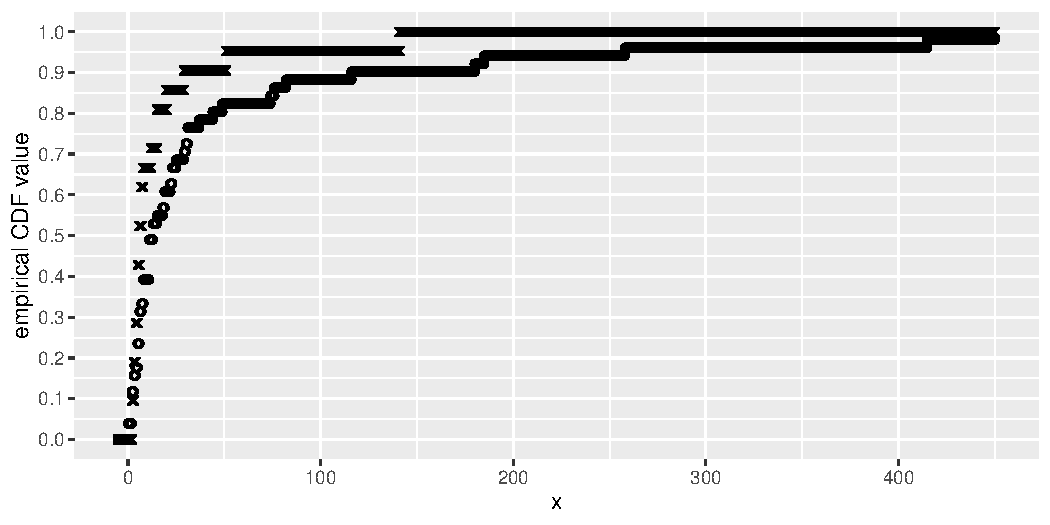
\includegraphics[width=6in]{empirical_cdfs}
\end{figure}
\vspace{-0.5cm}

Run the 2-sample KS test at $\alpha = 5\%$. Note that $F_K(1.359) = 95\%$ where $K \sim $ Kolmogorov dist. The alternative hypothesis is $H_a: \text{DGP}_1 \neq \text{DGP}_2$. Calculate the test statistic, provide the RET region, indicate and decision and write a concluding sentence.\spc{6}

\end{enumerate}

\problem Assume the following DGP:

\beqn
\Xoneton \iid \poisson{\theta_1} := \frac{\theta^x e^{-\theta}}{x!} \indic{x \in \naturals_0}
\eeqn


%\problem Assume you have data from two populations realized from the following DGPs:
%
%\beqn
%&& X_{1,1}, X_{1,2}, \ldots, X_{1, n_1} \iid \poisson{\theta_1} := \frac{\theta_1^x e^{-\theta_1}}{x!} \indic{x \in \naturals_0} \\
%&& X_{2,1}, X_{2,2}, \ldots, X_{2, n_2} \iid \poisson{\theta_2} := \frac{\theta_2^x e^{-\theta_2}}{x!} \indic{x \in \naturals_0} 
%\eeqn

Here are some facts about this DGP from the previous midterm:

\beqn
\mathcal{L}(\theta; \Xoneton) &=& \frac{\theta^{\sum_{i=1}^n X_i} e^{-n\theta}}{\prod_{i=1}^n X_i!} \\
\ell(\theta; \Xoneton) &=& \natlog{\theta} \sum_{i=1}^n X_i - n\theta - \sum_{i=1}^n \natlog{X_i!} \\
s(\theta; \Xoneton) &=& \frac{\sum_{i=1}^n X_i}{\theta} - n = n\parens{\frac{\Xbar}{\theta} - 1} \\
I_n(\theta) &=& \frac{n}{\theta}~~\Rightarrow~~I(\theta) = \frac{1}{\theta} \\
\thetahatmle &=& \Xbar~~\text{and it is the UMVUE, i.e.}~~\var{\Xbar} = \text{CRLB} :=  \oneover{I_n(\theta)} = \overn{\theta}
\eeqn
\vspace{-0.75cm}

\begin{enumerate}[(a)]

\subquestionwithpoints{6} Provide the score test statistic for testing $H_a: \theta \neq \theta_0$. The statistic must be a function of $\Xoneton, n, \theta_0$ only.  \spc{5}

\subquestionwithpoints{6} Provide the likelihood ratio test statistic $\hat{\Lambda} := 2\natlog{\hat{LR}}$ for testing $H_a: \theta \neq \theta_0$.  The statistic must be a function of $\Xoneton, n, \theta_0$ only.\spc{5}


\subquestionwithpoints{6} Consider the reparameterization of $\phi = \sqrt{\theta}$. Provide an asymptotically normal test statistic for testing $H_a: \phi \neq \phi_0$.  The statistic must be a function of $\Xoneton, n, \theta_0$ only.\spc{3}


For the rest of this problem, consider the prepandemic LIRR delay data where $n=51$ and $\xbar = 49.8$.

\subquestionwithpoints{6} Use the likelihood ratio test to test if $H_a: \theta \neq 35$. Indicate the RET region and the decision.\spc{6}

\subquestionwithpoints{6} Create a 95\% confidence interval estimate for $\phi = \sqrt{\theta}$.\spc{6}

\end{enumerate}

\problem We seek to test if hair length and eye color of cats are dependent. Here is a sample of cats organized into a contingency table with rowsums and colsums supplied:

\begin{table}[htp]
\centering
\begin{tabular}{c|ccc|c}
                & Blue Eyes & Yellow Eyes & Green Eyes & Total \\ \hline
Short Hair  & 25           & 48              &  13             & 86 \\
Long Hair   & 8            & 32              &  24             & 64 \\ \hline
Total         & 33           & 80              &  37             & 150 \\ 
\end{tabular}
\end{table}

Let $\theta_{i,j}$ denote the joint probability of having hair length of row $i$ and eye color of column $j$. Let $\theta_{i \cdot}$ denote the marginal probability of having hair length of row $i$. Let $\theta_{\cdot j}$ denote the marginal probability of having eye color of column $j$. 

Below are some 95\%iles of different chi-squared distributions by degrees of freedom.

\begin{table}[htp]
\centering
\begin{tabular}{c|ccccccccccc}
degrees of freedom &       1 & 2 & 3 & 4 & 5 & 6 & 7 & 8 & 9 & 10 \\ \hline
$x$ where $F_{\chi^2}(x) = .95$ & 3.84 & 5.99 & 7.81 & 9.49 & 11.07 & 12.59 & 14.07 & 15.51 & 16.92 & 18.31
\end{tabular}
\end{table}

\begin{enumerate}[(a)]

\subquestionwithpoints{3} Using the $\theta$ notation above, write the null and alternative hypotheses.\spc{3}

\subquestionwithpoints{10} Run the test from part (a) at $\alpha = 5\%$. Indicate the decision.\spc{20}

\end{enumerate}

\problem In class we modeled the maximum daily wind speed at JFK in the year 2013 and thus $n = 365$ for our dataset $\x$. We fit seven different models to the data by computing the MLE's of all their parameters and calculated their AIC's below from lowest to highest left to right.

\begin{table}[htp]
\centering
\begin{tabular}{c|ccccccccccc}
distribution    &gamma    & logistic     & normal   & gumbel  & weibull  &  frechet & gompertz      & exponential \\ \hline \hline
$k := \dime{\thetavec}$ & 2 & 2 & 2 & 2 & 2 & 2 & 2 & 1 \\
AIC  & 2262.6   & 2265.3     & 2289.4   & 2290.6   & 2300.2   & 2352.7  & 2404.5   & 2872.2 \\ \hline
Normalized  \\
Akaike \\
Weight &    0.799  &  0.201  &  0.000  &  0.000 &   0.000  &  0.000  &  0.000  &  0.000 
\end{tabular}
\end{table}

\begin{enumerate}[(a)]

\subquestionwithpoints{3} Which DGP of the seven is the best fitting model and why?\spc{4}

\subquestionwithpoints{3} Compute the corrected AIC for the best fitting model.\spc{3}

\subquestionwithpoints{6} Compute $\ell(\thetahathatmle; \x)$ where the DGP is $\Xoneton \iid \exponential{\theta}$.\spc{20}


\end{enumerate}



\end{document}
